% Methodology presentation
% Figures: figures_en/*.pdf (exported from the Graphviz .dot files) and interface_screenshot_*.png
% Compile with pdfLaTeX or XeLaTeX (XeLaTeX gives the Fira fonts of the metropolis theme).
\documentclass[aspectratio=169,10pt]{beamer}

\usetheme[progressbar=frametitle, numbering=fraction]{metropolis}

\usepackage[utf8]{inputenc}
\usepackage[T1]{fontenc}
\usepackage{amsmath, amssymb}
\usepackage{booktabs}
\usepackage{graphicx}
\usepackage{tikz}
\usetikzlibrary{arrows.meta, positioning, fit, calc, decorations.pathreplacing}

% Colours
\definecolor{bleu}{HTML}{0B4F8A}
\definecolor{bleuclair}{HTML}{E9EEF4}
\definecolor{orange}{HTML}{C26A00}
\definecolor{orangeclair}{HTML}{FCEBD7}
\definecolor{vert}{HTML}{1E7A46}
\definecolor{gris}{HTML}{6A6A6A}
\setbeamercolor{frametitle}{bg=bleu}
\setbeamercolor{progress bar}{fg=orange}
\setbeamercolor{alerted text}{fg=orange}

\tikzset{
  bloc/.style={draw=gris, rounded corners=3pt, fill=bleuclair, minimum height=0.75cm,
               minimum width=2.6cm, align=center, font=\footnotesize},
  donnee/.style={draw=gris, fill=white, minimum height=0.7cm, align=center, font=\footnotesize},
  expert/.style={draw=gris, rounded corners=3pt, fill=white, minimum height=0.6cm,
                 minimum width=1.1cm, align=center, font=\footnotesize},
  actif/.style={fill=orangeclair, draw=orange, thick},
  fleche/.style={-{Stealth[length=2mm]}, gris, thick},
}

\title{AI-assisted pharmaceutical analysis of prescriptions}
\subtitle{Combining retrieval-augmented generation and a rule-based expert system --- Methodology}
\author{Isen Naiken \and Bastian Fouquier \and Mathieu Boulin \and Marie-Pierre Guenfoudi}
\institute{CHU Dijon Bourgogne, Dijon, France}
\date{}

\begin{document}

\maketitle

\begin{frame}{Outline}
  \setbeamertemplate{section in toc}[sections numbered]
  \tableofcontents
\end{frame}

% =====================================================================
\section{Aim and overview}
% =====================================================================

\begin{frame}{Aim}
  \begin{itemize}
    \item Pharmaceutical analysis checks each prescription against the patient profile: doses, contraindications, interactions, guidelines.
    \item It is time-consuming and depends on up-to-date knowledge.
  \end{itemize}
  \vspace{0.3cm}
  \textbf{Aim:} build a tool that proposes a pharmaceutical opinion for each patient,
  \begin{itemize}
    \item based on clinical guidelines (\alert{retrieval-augmented generation}),
    \item checked by deterministic rules written by pharmacists (\alert{expert system}),
    \item with a short justification and \alert{verifiable sources}.
  \end{itemize}
  \vspace{0.3cm}
  The pharmacist keeps the final decision.
\end{frame}

\begin{frame}{Pipeline overview}
  \centering
  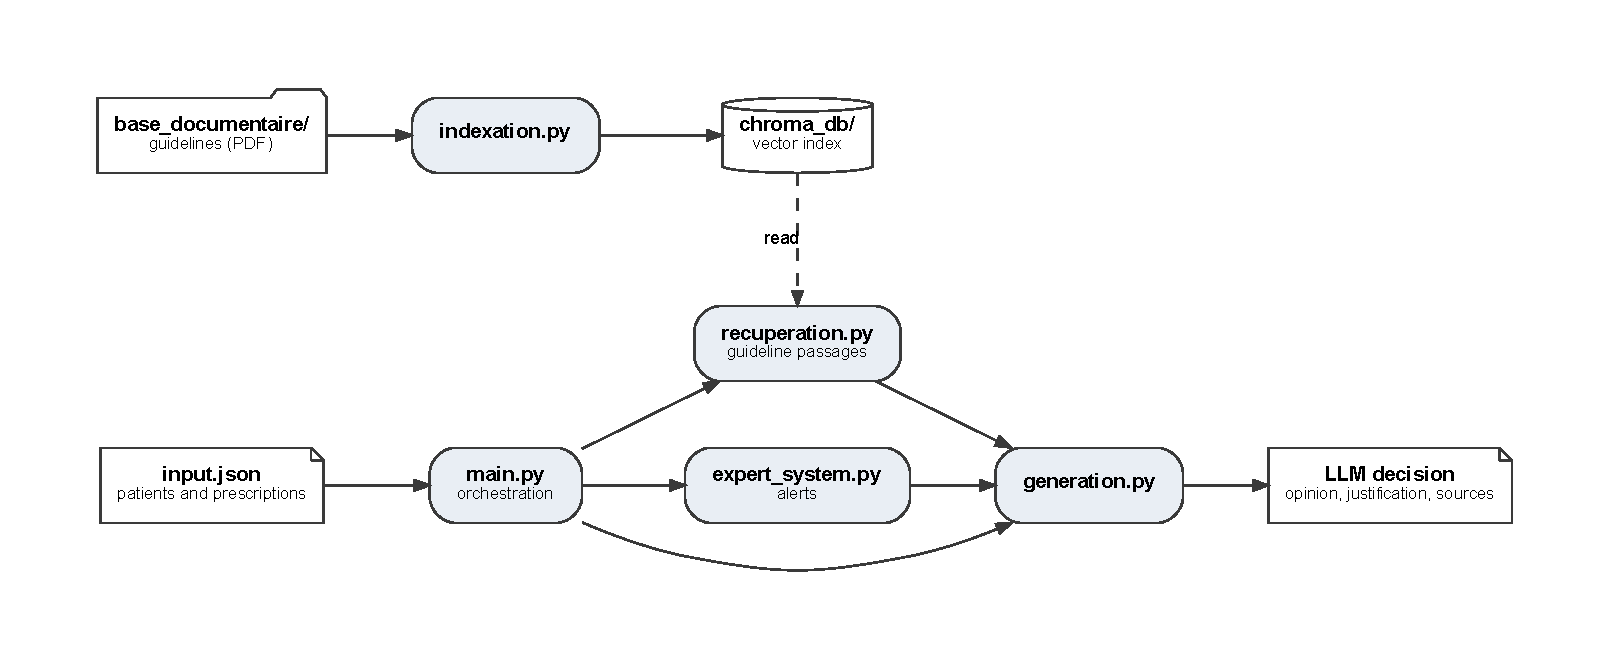
\includegraphics[width=\textwidth]{figures_en/figure_1.pdf}

  \vspace{0.3cm}
  \small Guidelines are indexed once. For each patient, the retrieval module and the expert system run first; their outputs are passed to the language model.
\end{frame}

\begin{frame}{Input data: the patient record}
  \begin{columns}[T]
    \begin{column}{0.42\textwidth}
      One JSON record per patient:
      \begin{itemize}
        \item identifier, age, sex, weight, height
        \item laboratory values (HbA1c, serum creatinine)
        \item prescription lines: INN, brand, dose, unit, dosage regimen, route
      \end{itemize}
      \vspace{0.2cm}
      \textbf{Example: PAT-0001}\\
      Woman, 95 years, 52 kg, 155 cm\\
      HbA1c 5\%, creatinine 70 $\mu$mol/L
    \end{column}
    \begin{column}{0.55\textwidth}
      \footnotesize
      \begin{tabular}{lrll}
        \toprule
        INN & Dose & Unit & Regimen \\
        \midrule
        glibenclamide & 5 & mg & 1 tab. morning and evening \\
        metformin & 1000 & mg & 1 tab. 3 times a day \\
        ramipril & 5 & mg & 1 tab. in the morning \\
        apixaban & 5 & mg & 1 tab. morning and evening \\
        bisoprolol & 2.5 & mg & 1 tab. in the morning \\
        paracetamol & 1 & g & up to 3 times a day if pain \\
        \bottomrule
      \end{tabular}
    \end{column}
  \end{columns}
\end{frame}

% =====================================================================
\section{Guideline indexing}
% =====================================================================

\begin{frame}{Guideline indexing}
  \begin{enumerate}
    \item \textbf{Text extraction:} each PDF is converted to text page by page (PyMuPDF4LLM, no OCR).
    \item \textbf{Splitting:} each page is split into passages of 1,500 characters, with a 200-character overlap.
    \item \textbf{Metadata:} each passage keeps its source file and page number.
    \item \textbf{Encoding:} each passage is turned into a vector with Qwen3-Embedding-8B.
    \item \textbf{Storage:} vectors are stored in ChromaDB, with the cosine distance.
  \end{enumerate}
  \vspace{0.3cm}
  \begin{center}
  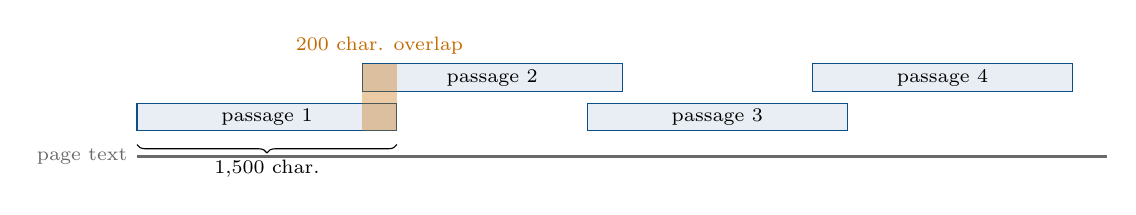
\begin{tikzpicture}[x=1.1cm, y=0.5cm]
    \draw[gris, thick] (0,0) -- (11.2,0);
    \node[font=\scriptsize, gris, anchor=east] at (0,0) {page text};
    \foreach \d/\l/\y in {0/1/1, 2.6/2/2, 5.2/3/1, 7.8/4/2} {
      \draw[fill=bleuclair, draw=bleu] (\d,\y-0.35) rectangle ++(3.0,0.7);
      \node[font=\scriptsize] at (\d+1.5,\y) {passage \l};
    }
    \draw[decorate, decoration={brace, amplitude=3pt, mirror}] (0,0.3) -- (3.0,0.3)
      node[midway, below=2pt, font=\scriptsize] {1,500 char.};
    \fill[orange, opacity=0.35] (2.6,0.65) rectangle (3.0,2.35);
    \node[font=\scriptsize, orange, above] at (2.8,2.35) {200 char. overlap};
  \end{tikzpicture}
  \end{center}
  \small The overlap avoids losing information cut at the border between two passages.
\end{frame}

% =====================================================================
\section{Background: embeddings and cosine similarity}
% =====================================================================

\begin{frame}{Text embeddings}
  \begin{itemize}
    \item An embedding model maps a text to a vector of real numbers:
      \[ \text{text} \;\longmapsto\; \mathbf{v} \in \mathbb{R}^d \]
    \item Texts with a similar meaning give vectors that point in a similar direction.
    \item The same model is used for the passages and for the queries, so they can be compared.
    \item In our pipeline: Qwen3-Embedding-8B, a transformer model trained for retrieval.
    \item Queries are preceded by a short task instruction, as recommended for this model:\\
      {\footnotesize\ttfamily Instruct: Retrieve medical guidelines useful to analyse this prescription}
  \end{itemize}
\end{frame}

\begin{frame}{Cosine similarity}
  \begin{columns}[c]
    \begin{column}{0.55\textwidth}
      The cosine similarity measures the angle $\theta$ between two vectors:
      \[
        \cos(\mathbf{q}, \mathbf{p}) \;=\; \frac{\mathbf{q}\cdot\mathbf{p}}{\lVert\mathbf{q}\rVert\,\lVert\mathbf{p}\rVert}
        \;=\; \frac{\sum_{i=1}^{d} q_i\,p_i}{\sqrt{\sum_{i} q_i^2}\,\sqrt{\sum_{i} p_i^2}}
      \]
      \begin{itemize}
        \item $1$: same direction (similar meaning)
        \item $0$: orthogonal (unrelated)
        \item $-1$: opposite direction
      \end{itemize}
      It depends only on the direction, not on the length of the vectors (e.g.\ the length of the text).
    \end{column}
    \begin{column}{0.42\textwidth}
      \centering
      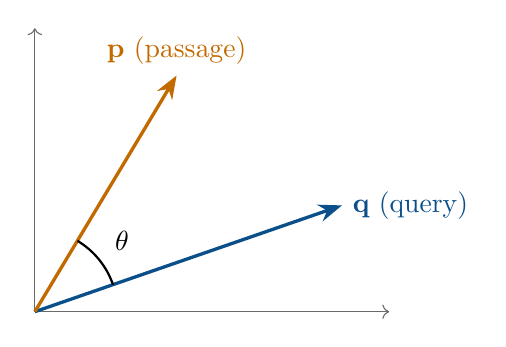
\begin{tikzpicture}[scale=1.5]
        \draw[->, gris] (0,0) -- (3,0);
        \draw[->, gris] (0,0) -- (0,2.4);
        \draw[-{Stealth}, very thick, bleu] (0,0) -- (2.6,0.9) node[right] {$\mathbf{q}$ (query)};
        \draw[-{Stealth}, very thick, orange] (0,0) -- (1.2,2.0) node[above] {$\mathbf{p}$ (passage)};
        \draw[thick] (19:0.7) arc (19:59:0.7);
        \node at (39:0.95) {$\theta$};
      \end{tikzpicture}
    \end{column}
  \end{columns}
\end{frame}

\begin{frame}{Cosine similarity: a small example}
  Query $\mathbf{q} = (1, 2, 0)$, two passages $\mathbf{p}_1 = (2, 4, 1)$ and $\mathbf{p}_2 = (0, 1, 3)$:
  \[
    \cos(\mathbf{q}, \mathbf{p}_1) = \frac{1\cdot2 + 2\cdot4 + 0\cdot1}{\sqrt{5}\,\sqrt{21}} = \frac{10}{10.25} \approx \alert{0.98}
    \qquad
    \cos(\mathbf{q}, \mathbf{p}_2) = \frac{0 + 2 + 0}{\sqrt{5}\,\sqrt{10}} = \frac{2}{7.07} \approx 0.28
  \]
  $\Rightarrow$ $\mathbf{p}_1$ is much closer to the query than $\mathbf{p}_2$.

  \vspace{0.4cm}
  \textbf{Cosine distance} (used by ChromaDB):
  \[ d(\mathbf{q}, \mathbf{p}) = 1 - \cos(\mathbf{q}, \mathbf{p}) \qquad d(\mathbf{q},\mathbf{p}_1) \approx 0.02, \quad d(\mathbf{q},\mathbf{p}_2) \approx 0.72 \]
  \textbf{Nearest-neighbour search:} for each query, keep the $k$ passages with the smallest distance (here $k = 3$).
  In practice, $d$ has thousands of dimensions and the search uses an approximate index (HNSW).
\end{frame}

% =====================================================================
\section{Retrieval of relevant passages}
% =====================================================================

\begin{frame}{Retrieval: one query per prescription line}
  \begin{columns}[c]
    \begin{column}{0.48\textwidth}
      \centering
      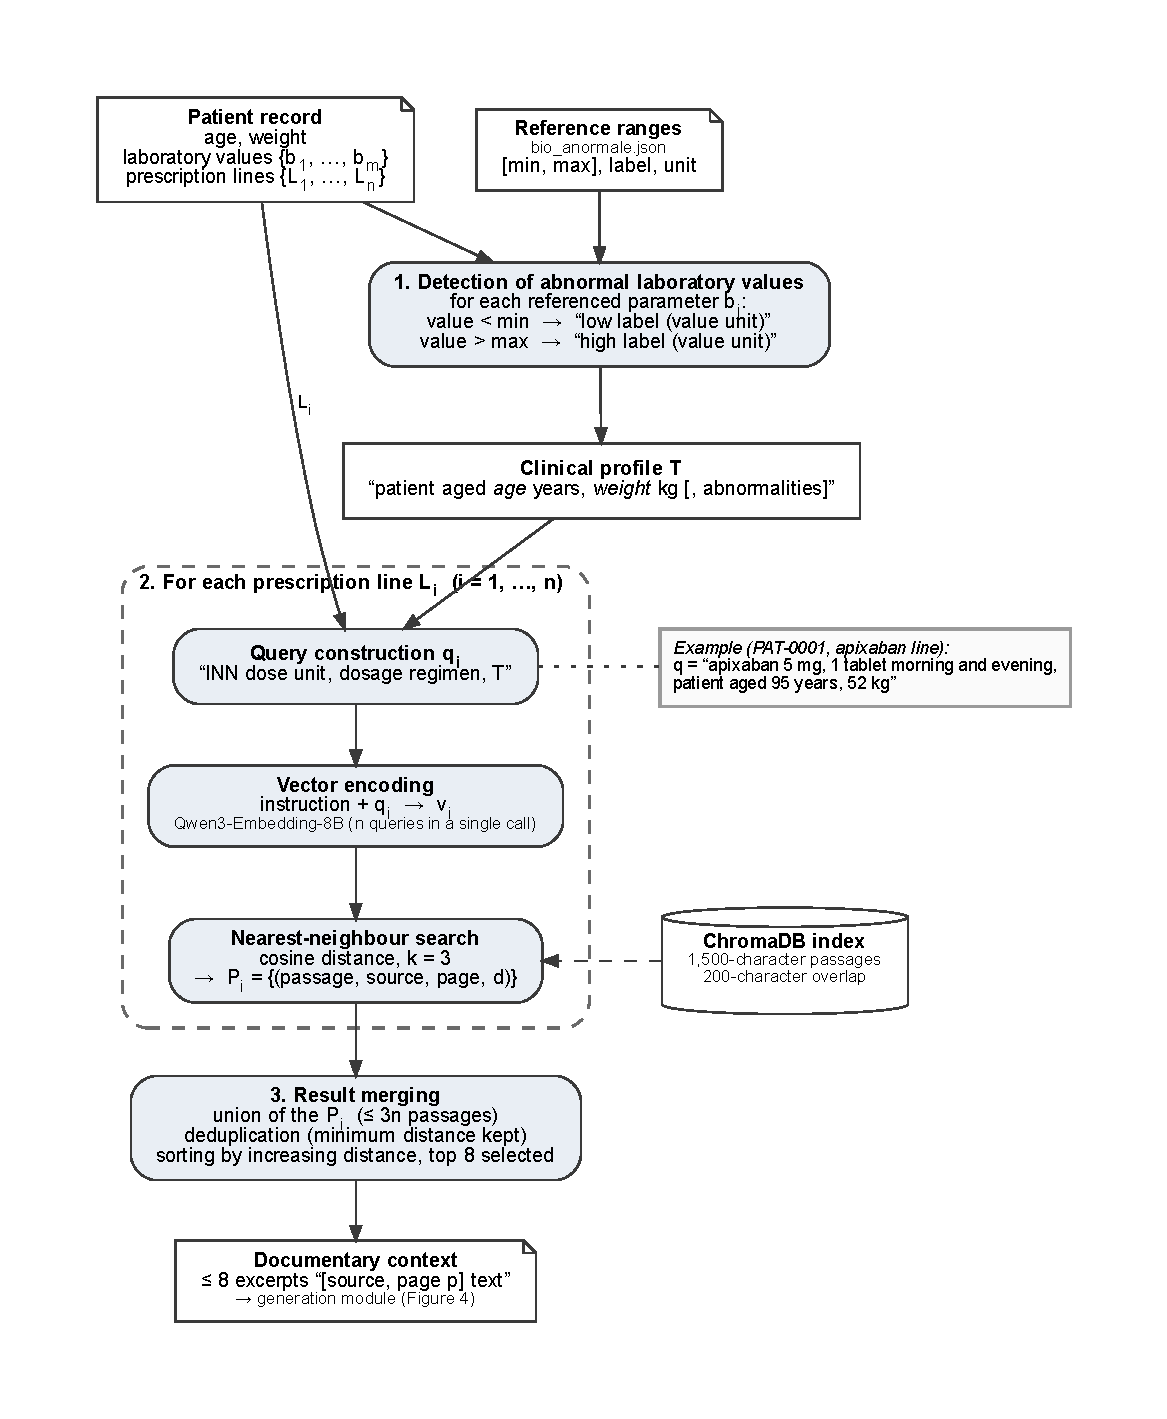
\includegraphics[height=0.82\textheight]{figures_en/figure_2.pdf}
    \end{column}
    \begin{column}{0.5\textwidth}
      \begin{enumerate}
        \item \textbf{Abnormal laboratory values} are detected with reference ranges set by pharmacists (e.g.\ creatinine 45--110 $\mu$mol/L) and added to the clinical profile.
        \item \textbf{One query per line:} drug, dose, regimen and clinical profile. Each query returns its 3 closest passages.
        \item \textbf{Merging:} duplicates removed, sorting by distance, the 8 closest passages are kept, with their source and page.
      \end{enumerate}
    \end{column}
  \end{columns}
\end{frame}

\begin{frame}{Retrieval: example for PAT-0001}
  Clinical profile: \emph{``patient aged 95 years, 52 kg''} (all laboratory values within range).

  \vspace{0.3cm}
  \footnotesize
  \begin{tabular}{ll}
    \toprule
    Line & Query $q_i$ \\
    \midrule
    1 & glibenclamide 5 mg, 1 tab. morning and evening, patient aged 95 years, 52 kg \\
    2 & metformin 1000 mg, 1 tab. 3 times a day, patient aged 95 years, 52 kg \\
    3 & ramipril 5 mg, 1 tab. in the morning, patient aged 95 years, 52 kg \\
    4 & apixaban 5 mg, 1 tab. morning and evening, patient aged 95 years, 52 kg \\
    5 & bisoprolol 2.5 mg, 1 tab. in the morning, patient aged 95 years, 52 kg \\
    6 & paracetamol 1 g, up to 3 times a day if pain, patient aged 95 years, 52 kg \\
    \bottomrule
  \end{tabular}

  \vspace{0.3cm}
  \normalsize
  6 queries $\times$ 3 passages = up to 18 candidates $\rightarrow$ duplicates removed $\rightarrow$ \alert{8 passages} sent to the LLM.
\end{frame}

% =====================================================================
\section{Rule-based expert system}
% =====================================================================

\begin{frame}{Expert system: deterministic rules}
  \begin{columns}[c]
    \begin{column}{0.5\textwidth}
      \centering
      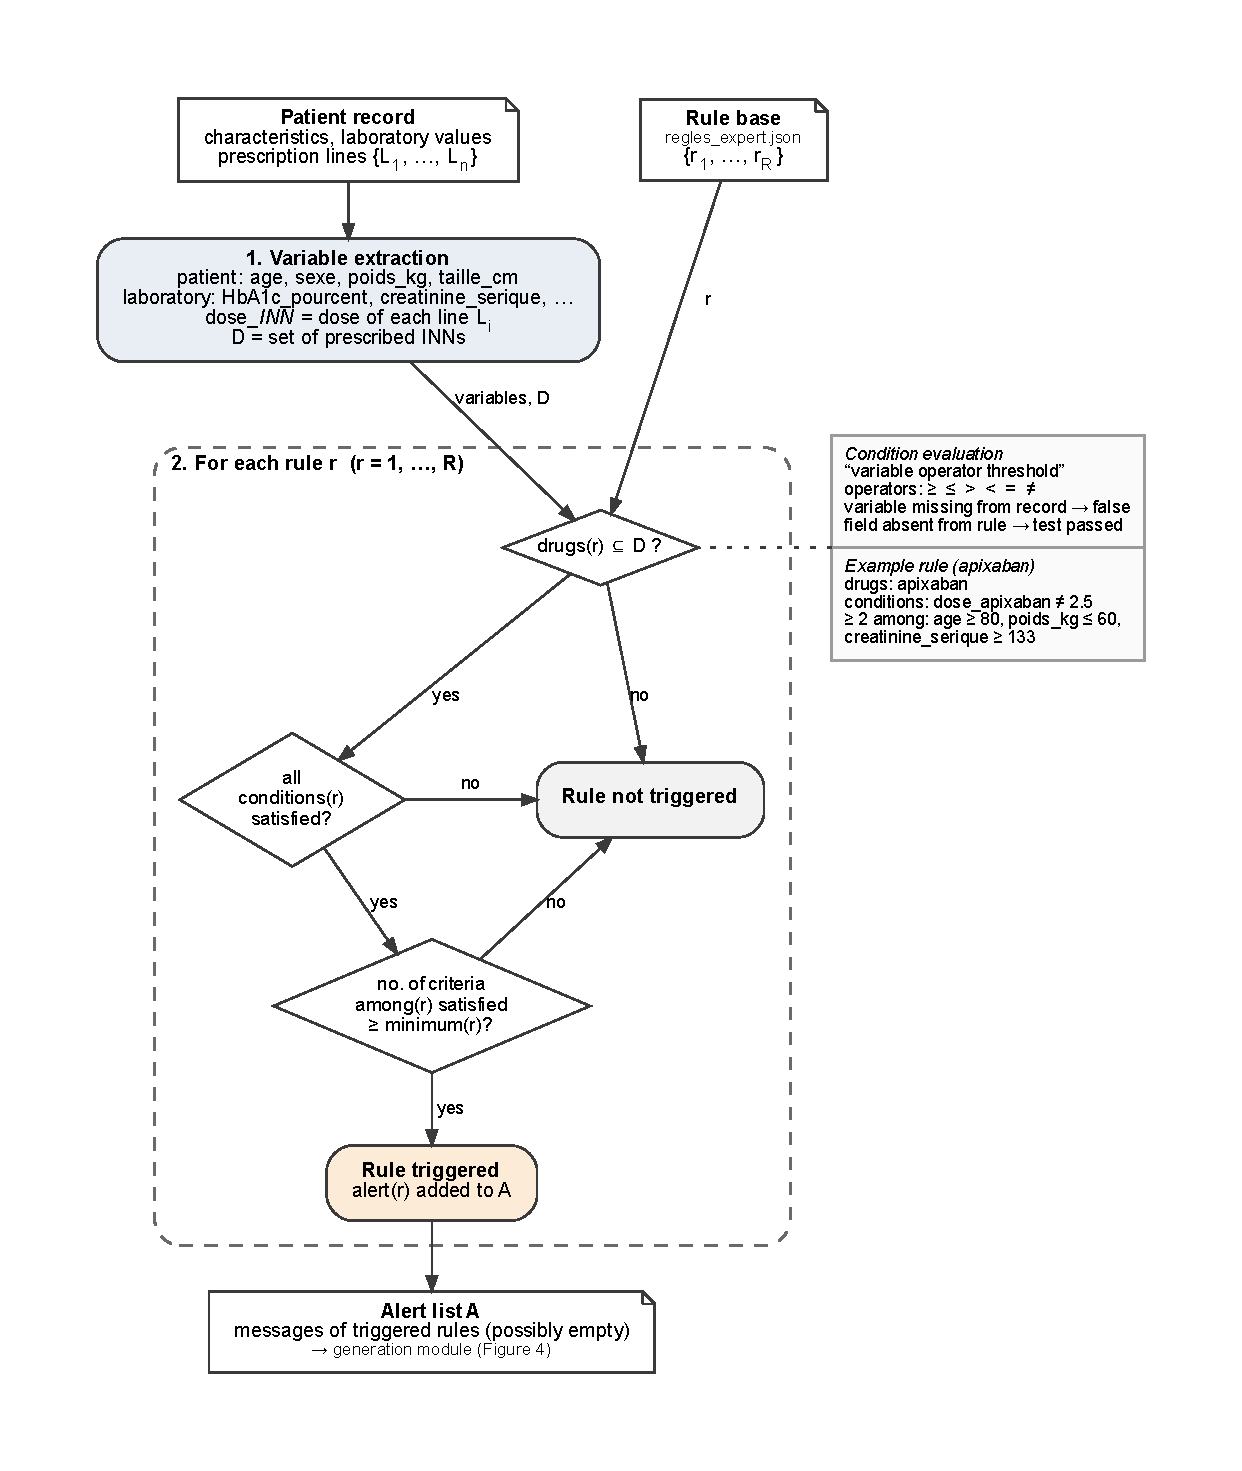
\includegraphics[height=0.82\textheight]{figures_en/figure_3.pdf}
    \end{column}
    \begin{column}{0.48\textwidth}
      A rule is triggered if:
      \begin{enumerate}
        \item all its target drugs are prescribed,
        \item all its mandatory conditions are true,
        \item at least \emph{minimum} of its optional criteria are true.
      \end{enumerate}
      \vspace{0.2cm}
      \begin{itemize}
        \item Rules are written in JSON by pharmacists, without programming.
        \item Same input $\Rightarrow$ same output: transparent and reproducible.
      \end{itemize}
    \end{column}
  \end{columns}
\end{frame}

\begin{frame}[fragile]{Expert system: example on PAT-0001}
  \begin{columns}[T]
    \begin{column}{0.5\textwidth}
      \textbf{Rule (regles\_expert.json)}
      \footnotesize
\begin{verbatim}
{
  "medicaments": ["apixaban"],
  "conditions": ["dose_apixaban != 2.5"],
  "parmi": ["age >= 80",
            "poids_kg <= 60",
            "creatinine_serique >= 133"],
  "minimum": 2,
  "alerte": "Apixaban: recommended dose
             is 2.5 mg twice a day ..."
}
\end{verbatim}
    \end{column}
    \begin{column}{0.48\textwidth}
      \textbf{Evaluation for PAT-0001}
      \small
      \begin{tabular}{ll}
        \toprule
        Test & Result \\
        \midrule
        apixaban prescribed & \textcolor{vert}{yes} \\
        dose $= 5 \neq 2.5$ & \textcolor{vert}{true} \\
        age $95 \geq 80$ & \textcolor{vert}{true} \\
        weight $52 \leq 60$ & \textcolor{vert}{true} \\
        creatinine $70 \geq 133$ & \textcolor{red}{false} \\
        criteria met: $2 \geq 2$ & \textcolor{vert}{true} \\
        \bottomrule
      \end{tabular}

      \vspace{0.3cm}
      $\Rightarrow$ \alert{Rule triggered}: the alert is sent to the LLM.
    \end{column}
  \end{columns}
\end{frame}

% =====================================================================
\section{Background: from RNNs to Mixture-of-Experts transformers}
% =====================================================================

\begin{frame}{Recurrent neural networks (RNN)}
  \begin{columns}[c]
    \begin{column}{0.5\textwidth}
      \begin{itemize}
        \item Read the text one token at a time.
        \item A hidden state $h_t$ summarises everything read so far:
          \[ h_t = \tanh(W_h\, h_{t-1} + W_x\, x_t + b) \]
        \item LSTM and GRU add gates to keep information longer.
      \end{itemize}
      \textbf{Limits}
      \begin{itemize}
        \item Sequential: cannot be parallelised over tokens.
        \item Long-range information fades in a single vector.
      \end{itemize}
    \end{column}
    \begin{column}{0.48\textwidth}
      \centering
      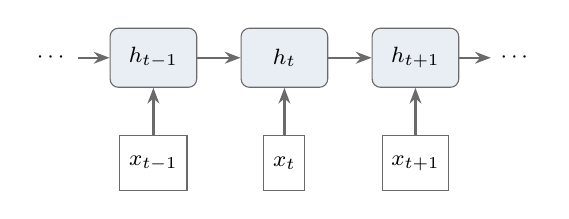
\begin{tikzpicture}[node distance=0.6cm and 0.55cm]
        \node[bloc, minimum width=1.1cm] (h1) {$h_{t-1}$};
        \node[bloc, minimum width=1.1cm, right=of h1] (h2) {$h_t$};
        \node[bloc, minimum width=1.1cm, right=of h2] (h3) {$h_{t+1}$};
        \node[donnee, below=of h1] (x1) {$x_{t-1}$};
        \node[donnee, below=of h2] (x2) {$x_t$};
        \node[donnee, below=of h3] (x3) {$x_{t+1}$};
        \node[left=0.4cm of h1, font=\footnotesize] (d) {$\cdots$};
        \node[right=0.4cm of h3, font=\footnotesize] (f) {$\cdots$};
        \draw[fleche] (d) -- (h1);
        \draw[fleche] (h1) -- (h2);
        \draw[fleche] (h2) -- (h3);
        \draw[fleche] (h3) -- (f);
        \foreach \i in {1,2,3} \draw[fleche] (x\i) -- (h\i);
      \end{tikzpicture}
    \end{column}
  \end{columns}
\end{frame}

\begin{frame}{The transformer layer}
  \begin{columns}[c]
    \begin{column}{0.55\textwidth}
      \begin{itemize}
        \item All tokens are processed in parallel.
        \item \textbf{Self-attention:} each token looks at all the other tokens:
          \[ \mathrm{Attention}(Q,K,V) = \mathrm{softmax}\!\left(\frac{QK^\top}{\sqrt{d_k}}\right) V \]
        \item \textbf{Feed-forward network (FFN):} the same small network is applied to each token. It holds most of the parameters (``knowledge'').
        \item Residual connections and normalisation around each block.
        \item An LLM stacks tens of these layers.
      \end{itemize}
    \end{column}
    \begin{column}{0.42\textwidth}
      \centering
      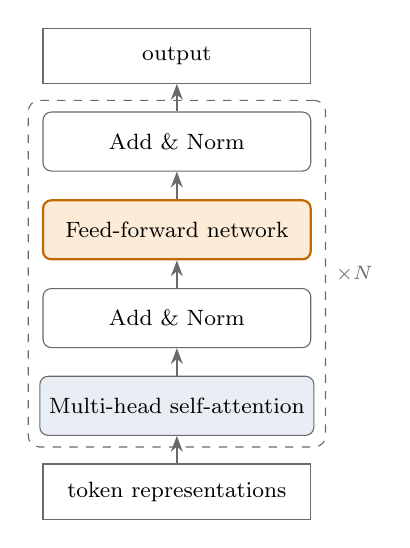
\begin{tikzpicture}[node distance=0.35cm]
        \node[donnee, minimum width=3.4cm] (in) {token representations};
        \node[bloc, minimum width=3.4cm, above=of in] (att) {Multi-head self-attention};
        \node[bloc, minimum width=3.4cm, above=of att, fill=white] (n1) {Add \& Norm};
        \node[bloc, minimum width=3.4cm, above=of n1, actif] (ffn) {Feed-forward network};
        \node[bloc, minimum width=3.4cm, above=of ffn, fill=white] (n2) {Add \& Norm};
        \node[donnee, minimum width=3.4cm, above=of n2] (out) {output};
        \draw[fleche] (in) -- (att);
        \draw[fleche] (att) -- (n1);
        \draw[fleche] (n1) -- (ffn);
        \draw[fleche] (ffn) -- (n2);
        \draw[fleche] (n2) -- (out);
        \node[draw=gris, dashed, rounded corners, fit=(att)(n2), inner sep=4pt,
              label={[font=\scriptsize, gris]right:$\times N$}] {};
      \end{tikzpicture}
    \end{column}
  \end{columns}
\end{frame}

\begin{frame}{Mixture of Experts (MoE)}
  \begin{columns}[c]
    \begin{column}{0.5\textwidth}
      \begin{itemize}
        \item Replace one large network by $N$ smaller \textbf{experts} $E_1, \dots, E_N$.
        \item A \textbf{router} chooses, for each token, the $k$ most suitable experts (top-$k$):
          \[ g(x) = \mathrm{softmax}\big(\mathrm{TopK}(W_r\, x)\big) \]
          \[ y = \sum_{i \in \mathrm{TopK}(x)} g_i(x)\; E_i(x) \]
        \item Only $k$ experts are computed per token: \alert{sparse} activation.
        \item An auxiliary loss balances the load between experts.
      \end{itemize}
    \end{column}
    \begin{column}{0.48\textwidth}
      \centering
      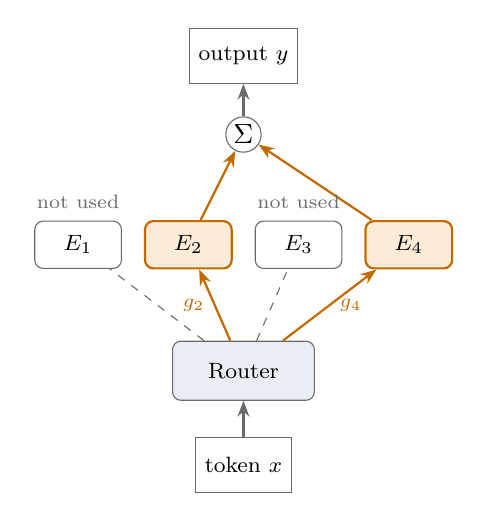
\begin{tikzpicture}
        \node[donnee] (x) at (0,0) {token $x$};
        \node[bloc, minimum width=1.8cm] (r) at (0,1.2) {Router};
        \node[expert] (e1) at (-2.1,2.8) {$E_1$};
        \node[expert, actif] (e2) at (-0.7,2.8) {$E_2$};
        \node[expert] (e3) at (0.7,2.8) {$E_3$};
        \node[expert, actif] (e4) at (2.1,2.8) {$E_4$};
        \node[circle, draw=gris, inner sep=1pt] (s) at (0,4.2) {$\Sigma$};
        \node[donnee] (y) at (0,5.2) {output $y$};
        \draw[fleche] (x) -- (r);
        \draw[gris, dashed] (r) -- (e1);
        \draw[gris, dashed] (r) -- (e3);
        \draw[fleche, orange] (r) -- node[left, font=\scriptsize] {$g_2$} (e2);
        \draw[fleche, orange] (r) -- node[right, font=\scriptsize] {$g_4$} (e4);
        \draw[fleche, orange] (e2) -- (s);
        \draw[fleche, orange] (e4) -- (s);
        \draw[fleche] (s) -- (y);
        \node[font=\scriptsize, gris] at (-2.1,3.35) {not used};
        \node[font=\scriptsize, gris] at (0.7,3.35) {not used};
      \end{tikzpicture}

      \small Example with $N = 4$ experts and $k = 2$.
    \end{column}
  \end{columns}
\end{frame}

\begin{frame}{MoE in RNNs and in transformers}
  \begin{columns}[T]
    \begin{column}{0.48\textwidth}
      \textbf{MoE between RNN layers}\\
      \small (Shazeer et al., 2017)
      \begin{itemize}
        \item MoE layer placed between two stacked LSTM layers.
        \item Applied at each time step.
        \item Thousands of experts, models up to 137B parameters for translation and language modelling.
      \end{itemize}
      \centering
      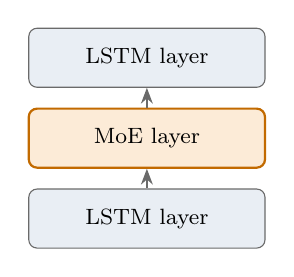
\begin{tikzpicture}[node distance=0.25cm]
        \node[bloc, minimum width=3cm] (l1) {LSTM layer};
        \node[bloc, minimum width=3cm, above=of l1, actif] (m) {MoE layer};
        \node[bloc, minimum width=3cm, above=of m] (l2) {LSTM layer};
        \draw[fleche] (l1) -- (m);
        \draw[fleche] (m) -- (l2);
      \end{tikzpicture}
    \end{column}
    \begin{column}{0.48\textwidth}
      \textbf{MoE inside transformer layers}\\
      \small (GShard, Switch Transformer, Mixtral, Qwen3)
      \begin{itemize}
        \item The FFN of each layer is replaced by an MoE layer.
        \item Self-attention is unchanged and shared by all tokens.
        \item Standard design of large modern LLMs.
      \end{itemize}
      \centering
      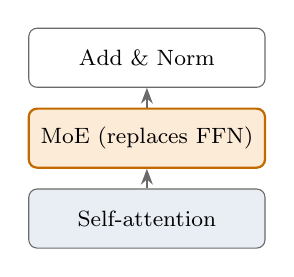
\begin{tikzpicture}[node distance=0.25cm]
        \node[bloc, minimum width=3cm] (a) {Self-attention};
        \node[bloc, minimum width=3cm, above=of a, actif] (m) {MoE (replaces FFN)};
        \node[bloc, minimum width=3cm, above=of m, fill=white] (n) {Add \& Norm};
        \draw[fleche] (a) -- (m);
        \draw[fleche] (m) -- (n);
      \end{tikzpicture}
    \end{column}
  \end{columns}
\end{frame}

\begin{frame}{Why an MoE model in our pipeline?}
  \textbf{Qwen3.6-35B-A3B}
  \begin{itemize}
    \item \textbf{35B} parameters in total: large capacity to store medical knowledge.
    \item \textbf{A3B}: only about \textbf{3B} parameters are \emph{activated} for each token.
  \end{itemize}
  \vspace{0.3cm}
  \begin{tabular}{lcc}
    \toprule
     & Dense 35B model & MoE 35B-A3B \\
    \midrule
    Parameters stored in memory & 35B & 35B \\
    Parameters used per token & 35B & $\approx$ 3B \\
    Compute per token & high & close to a 3B model \\
    \bottomrule
  \end{tabular}
  \vspace{0.3cm}
  \begin{itemize}
    \item Fast and cheap inference, while keeping the knowledge of a large model.
    \item Limit: all experts must still be loaded in memory.
  \end{itemize}
\end{frame}

% =====================================================================
\section{Generation of the pharmaceutical opinion}
% =====================================================================

\begin{frame}{Generation by the LLM}
  \centering
  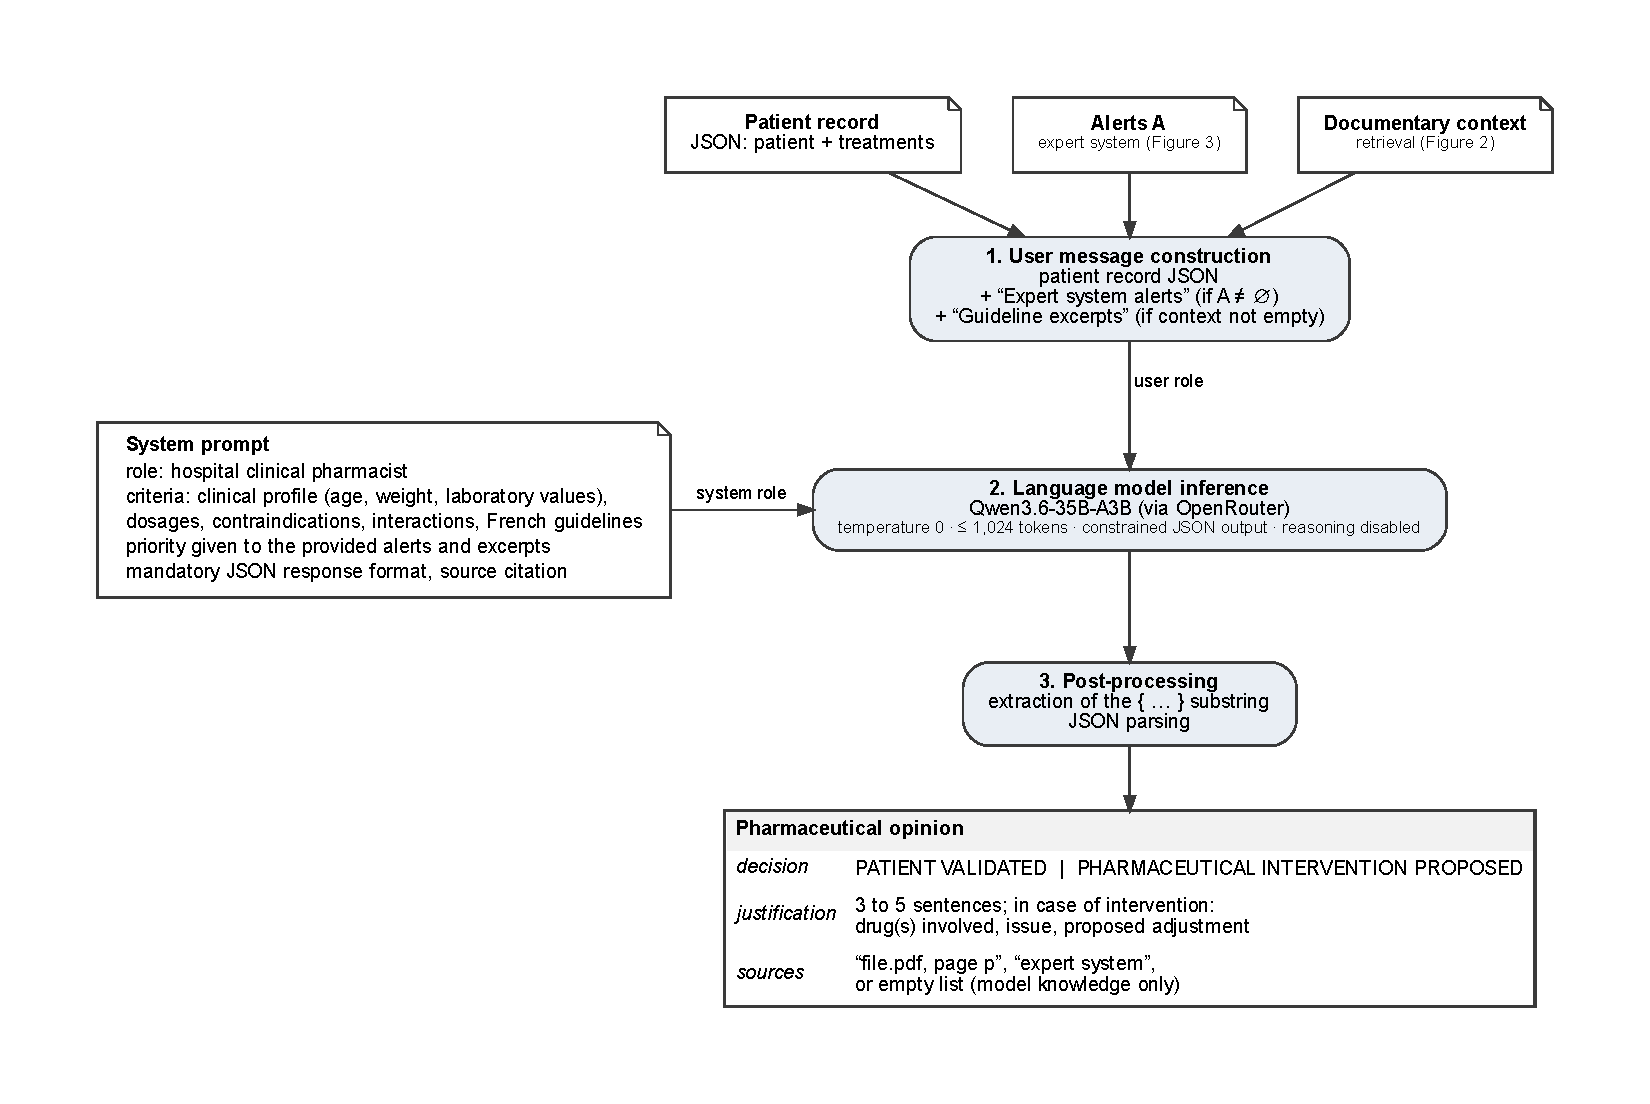
\includegraphics[height=0.62\textheight]{figures_en/figure_4.pdf}

  \small
  \begin{itemize}
    \item User message: patient record (JSON) + expert system alerts + retrieved passages.
    \item Qwen3.6-35B-A3B via OpenRouter, temperature 0, at most 1,024 tokens, JSON output, reasoning disabled.
  \end{itemize}
\end{frame}

\begin{frame}{System prompt and output}
  \begin{columns}[T]
    \begin{column}{0.48\textwidth}
      \textbf{System prompt}
      \begin{itemize}
        \item Act as a hospital clinical pharmacist.
        \item Consider age, weight, laboratory values, doses, contraindications, interactions, French guidelines.
        \item Rely first on the alerts and passages provided.
        \item Answer only in JSON and cite the sources.
      \end{itemize}
    \end{column}
    \begin{column}{0.48\textwidth}
      \textbf{Output}
      \begin{itemize}
        \item \texttt{decision}: patient validated \emph{or} pharmaceutical intervention proposed
        \item \texttt{justification}: 3 to 5 sentences (drugs involved, problem, proposed change)
        \item \texttt{sources}: ``file.pdf, page $p$'', ``expert system'', or empty
      \end{itemize}
    \end{column}
  \end{columns}
  \vspace{0.3cm}
  \textbf{PAT-0001:} \alert{intervention proposed}: reduce apixaban to 2.5 mg twice a day (expert system); stop glibenclamide because of the risk of severe hypoglycaemia in an elderly patient (SFD guidelines, pages 27--28); review the metformin dose.
\end{frame}

% =====================================================================
\section{Graphical interface}
% =====================================================================

\begin{frame}{Graphical interface: results}
  \centering
  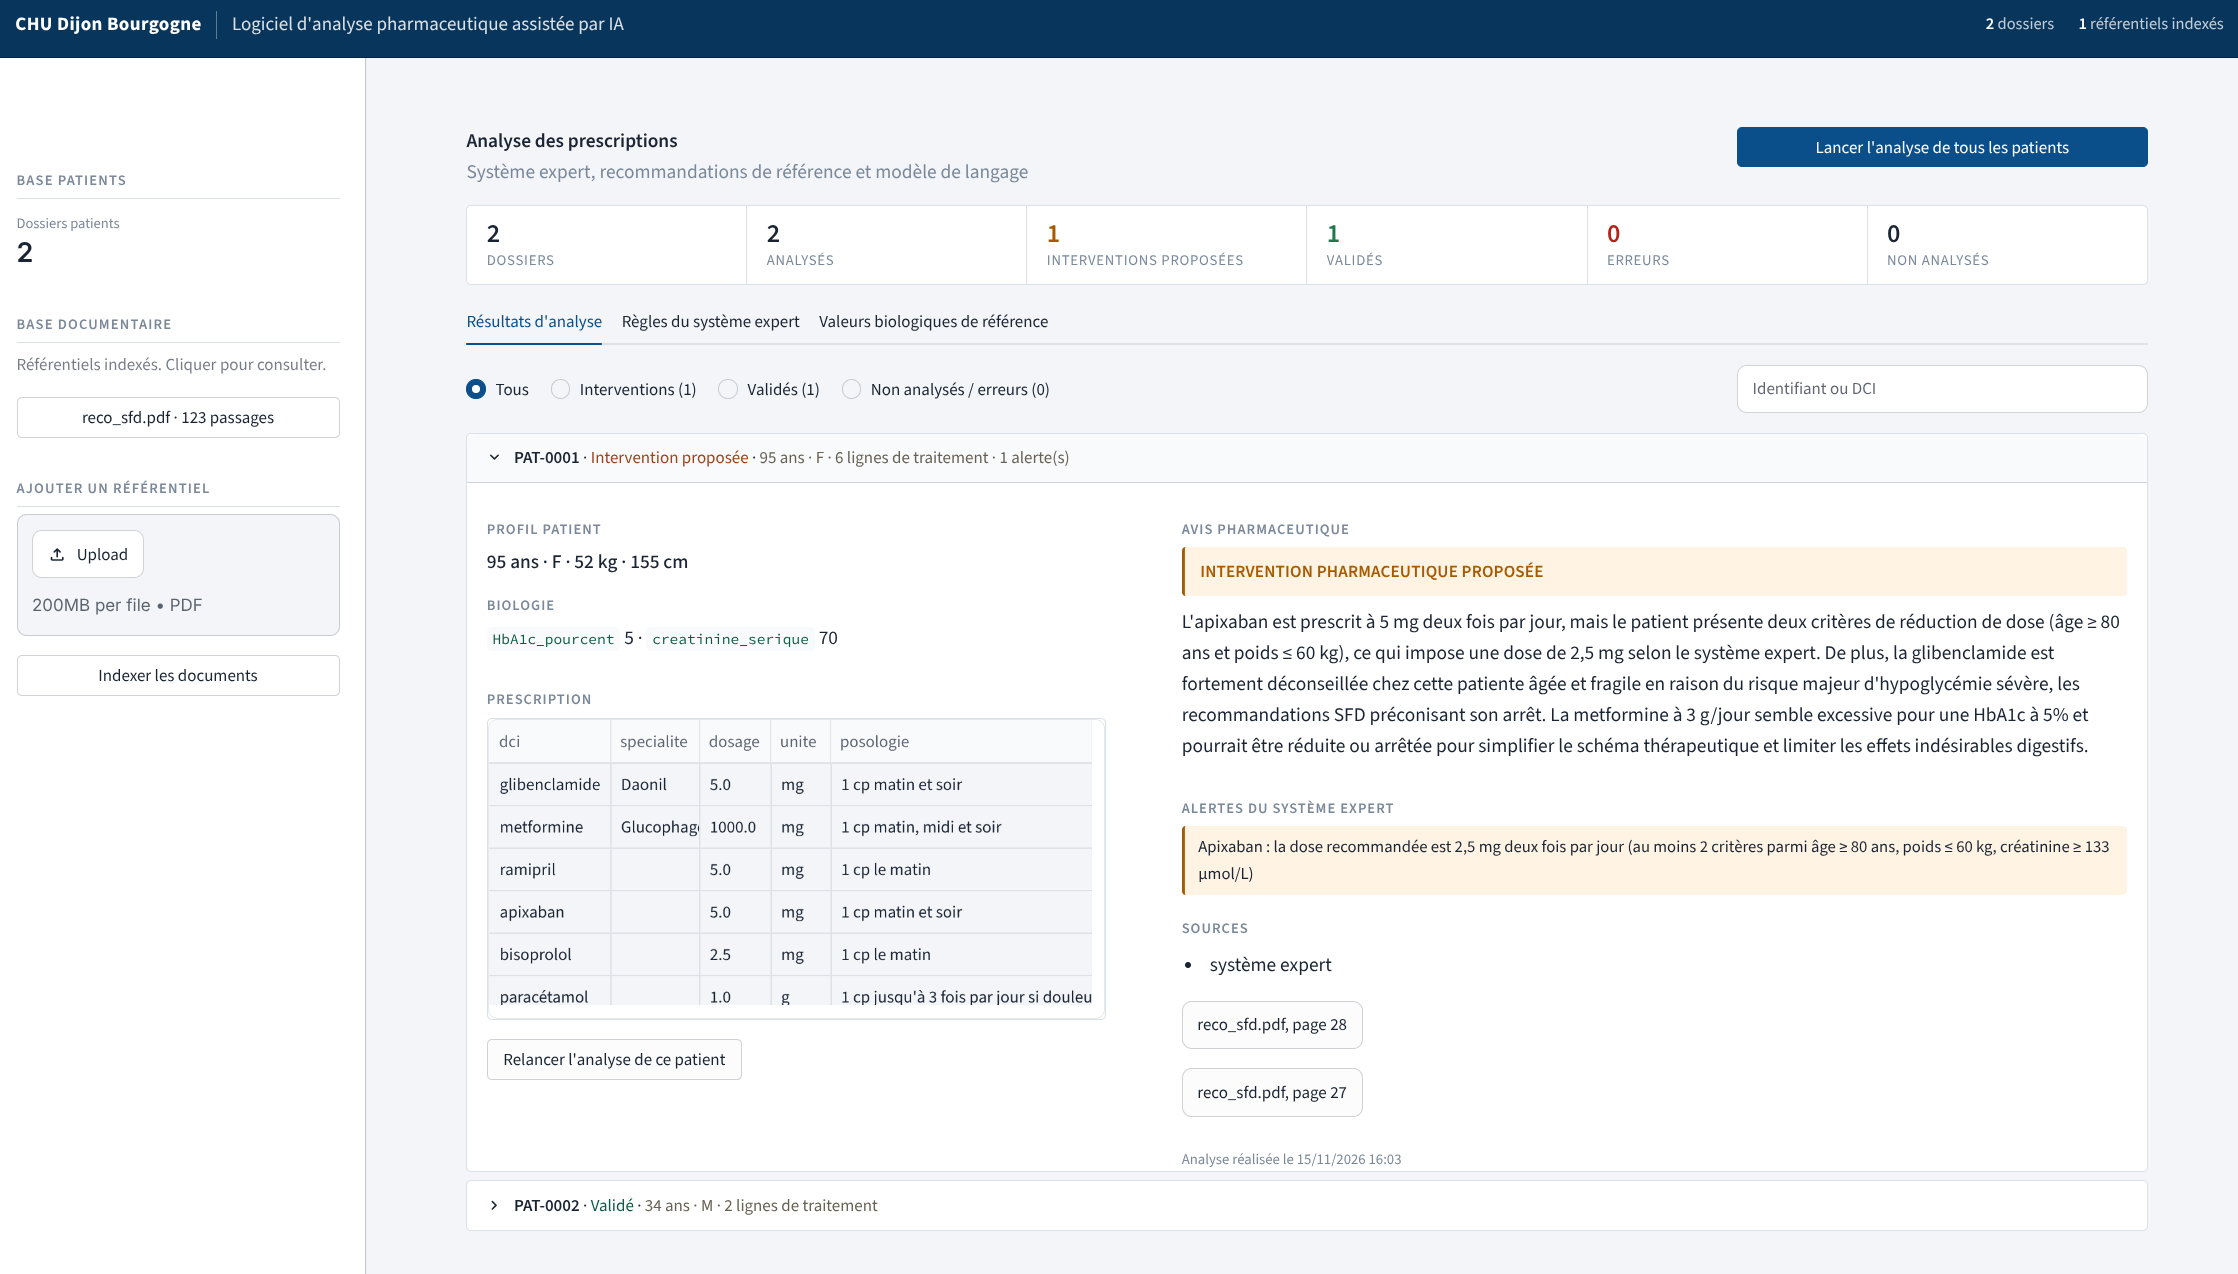
\includegraphics[height=0.78\textheight]{interface_screenshot_1.png}

  \small Patient profile, prescription, opinion, expert system alerts and clickable sources.
\end{frame}

\begin{frame}{Graphical interface: source checking}
  \centering
  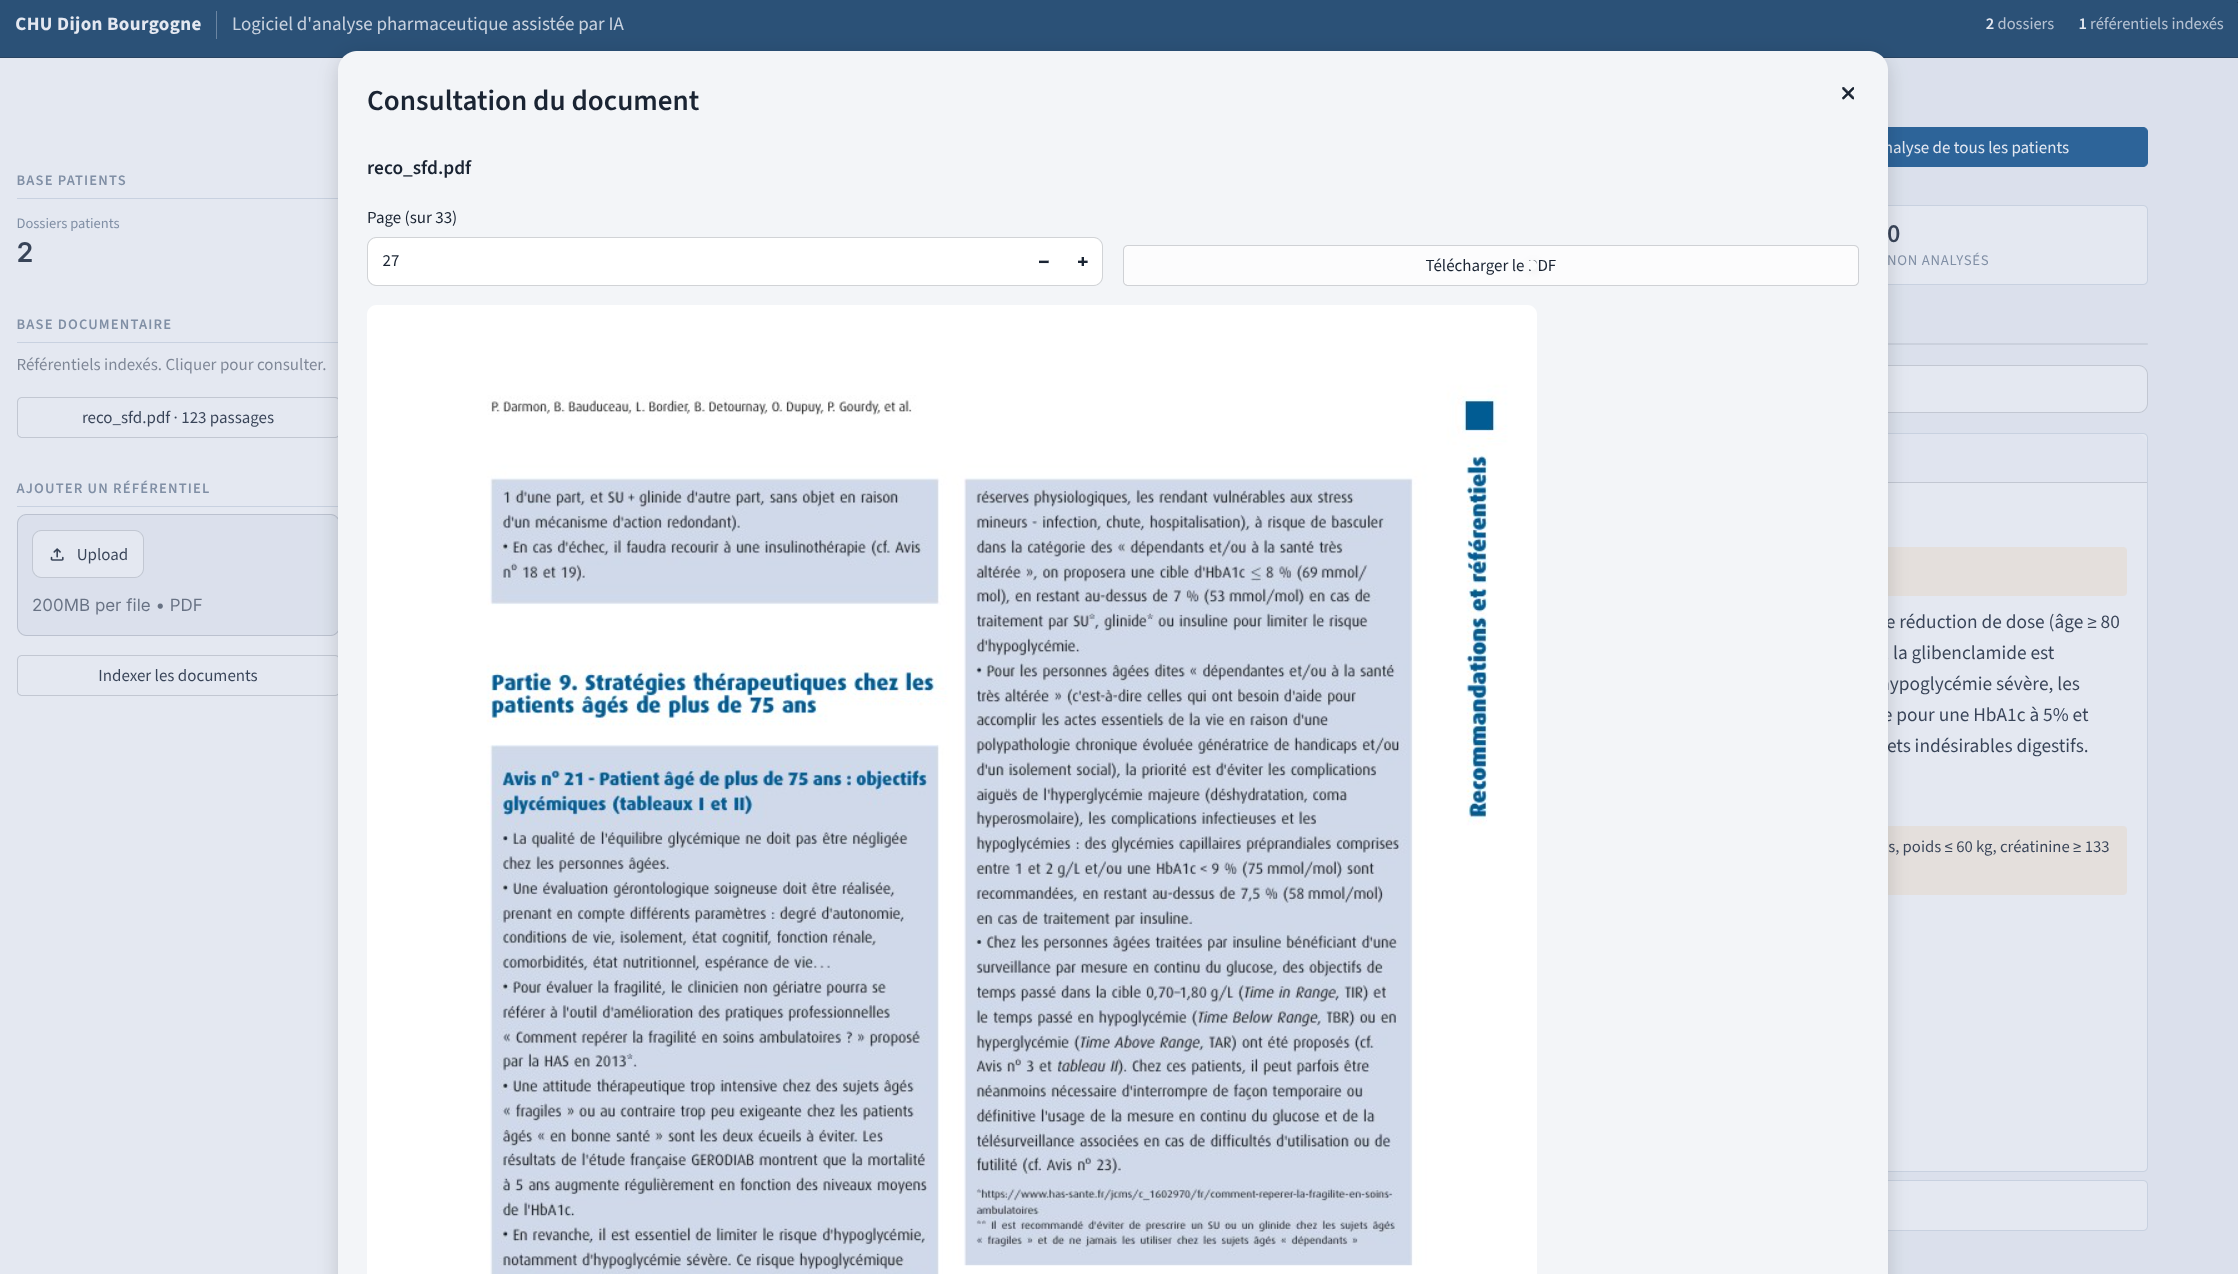
\includegraphics[height=0.78\textheight]{interface_screenshot_2.png}

  \small One click on a source opens the guideline at the page cited by the model.
\end{frame}

% =====================================================================
\section*{Summary}
% =====================================================================

\begin{frame}{Summary}
  \begin{itemize}
    \item \textbf{Retrieval:} one query per prescription line, cosine similarity, 8 guideline passages with source and page.
    \item \textbf{Expert system:} deterministic rules written by pharmacists, transparent and reproducible.
    \item \textbf{Generation:} MoE LLM (35B total, 3B active), temperature 0, structured JSON opinion.
    \item \textbf{Interface:} analysis, verification of sources, editing of rules and reference ranges without programming.
  \end{itemize}
  \vspace{0.4cm}
  \textbf{Next steps:} evaluation on a larger set of patients, comparison with pharmacists' decisions, more guidelines and rules.
\end{frame}

\begin{frame}[allowframebreaks]{References}
  \footnotesize
  \begin{itemize}
    \item Jacobs R.A., Jordan M.I., Nowlan S.J., Hinton G.E. Adaptive mixtures of local experts. \emph{Neural Computation}, 1991.
    \item Hochreiter S., Schmidhuber J. Long short-term memory. \emph{Neural Computation}, 1997.
    \item Shazeer N. et al. Outrageously large neural networks: the sparsely-gated mixture-of-experts layer. \emph{ICLR}, 2017.
    \item Vaswani A. et al. Attention is all you need. \emph{NeurIPS}, 2017.
    \item Lewis P. et al. Retrieval-augmented generation for knowledge-intensive NLP tasks. \emph{NeurIPS}, 2020.
    \item Lepikhin D. et al. GShard: scaling giant models with conditional computation and automatic sharding. \emph{ICLR}, 2021.
    \item Fedus W., Zoph B., Shazeer N. Switch Transformers: scaling to trillion parameter models with simple and efficient sparsity. \emph{JMLR}, 2022.
    \item Jiang A.Q. et al. Mixtral of experts. \emph{arXiv:2401.04088}, 2024.
    \item Malkov Y.A., Yashunin D.A. Efficient and robust approximate nearest neighbor search using HNSW graphs. \emph{IEEE TPAMI}, 2020.
  \end{itemize}
\end{frame}

\end{document}
